\newpage
\section{Casi d'uso}
testo

	\subsection{Introduzione}
	testo
	
	\subsection{Attori}
	\begin{itemize}
		\item Producer
		\item Utente che interagisce con il gestore personale
		\item Consumer (secondario)
	\end{itemize}
	
	\subsection{Elenco casi d'uso}

%TODO: da ricordarsi: se qualcuno è offline, c'è la possibilità che il messaggio venga perso.

\newcounter{uccount}

\stepcounter{uccount}
\subsubsection{UC\theuccount\ - Redmine/GitLab genera una segnalazione}
    \begin{figure}[H]
		\centering
		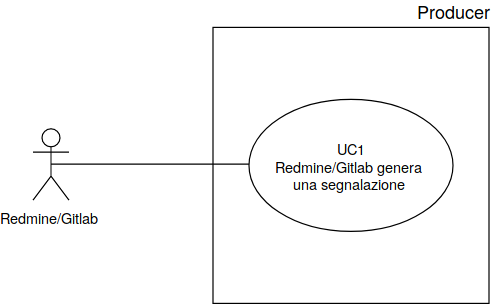
\includegraphics[width=0.7\textwidth]{img/UC1.png}\\
		\caption{UC\theuccount - Redmine/GitLab genera una segnalazione}
	\end{figure}
	\begin{itemize}
		\item \textbf{Codice}: UC\theuccount.
		\item \textbf{Titolo}: Redmine/GitLab genera una segnalazione.
		\item \textbf{Attori primari}: Redmine/Gitlab.
		\item \textbf{Descrizione}:
		 il sistema qui è il Producer ed è interno al sistema Butterfly. Cambio stato repository tramite commit per GitLab. Cambio di stato issue tracking system per GitLab e Redmine.
		\item \textbf{Precondizione}: c'è qualcosa da segnalare
		\item \textbf{Postcondizione}: segnalazione generata e inviata
		\item \textbf{Scenario principale}: 
		\begin{enumerate}
			\item Redmine/GitLab prepara una segnalazione da mandare
			\item Redmine/GitLab invia la segnalazione al Producer.
		\end{enumerate}
		
	\end{itemize}

\subsubsection{UC\theuccount.1 - Redmine/GitLab crea e invia un messaggio per il Producer}
    \begin{figure}[H]
		\centering
		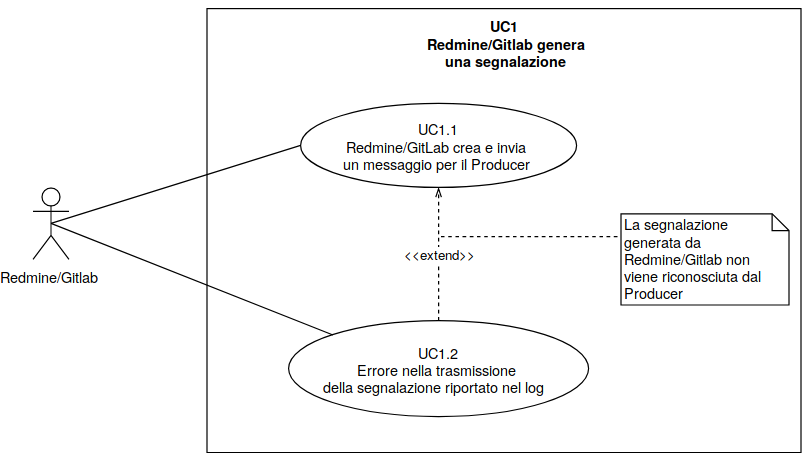
\includegraphics[width=1\textwidth]{img/UC1_1.png}\\
		\caption{UC\theuccount.1, UC\theuccount.2 - segnalazione corretta ed errata}
	\end{figure}
	\begin{itemize}
		\item \textbf{Codice}: UC\theuccount.1.
		\item \textbf{Titolo}: Redmine/GitLab crea e invia un messaggio per il Producer.
		\item \textbf{Attori primari}: Redmine/Gitlab.
		\item \textbf{Descrizione}:
		il sistema qui è il Producer ed è interno al sistema Butterfly. Cambio stato repository tramite commit per GitLab. Cambio di stato issue tracking system per GitLab e Redmine.
		\item \textbf{Precondizione}: Redmine/Gitlab generano un messaggio per il Producer
		\item \textbf{Postcondizione}: segnalazione generata e inviata al Producer
		\item \textbf{Scenario principale}: 
		\begin{enumerate}
			\item Redmine/GitLab prepara una segnalazione da mandare
			\item Redmine/GitLab invia la segnalazione al Producer.
		\end{enumerate}
		\item \textbf{Estensioni}: messaggio creato con parametri errati.
	\end{itemize}


%\subsubsection{UC\theuccount.2 - Redmine/GitLab genera una segnalazione errata}
\subsubsection{UC\theuccount.2 - Errore nella trasmissione della segnalazione}
	\begin{itemize}
		\item \textbf{Codice}: UC\theuccount.2.
		\item \textbf{Titolo}: Errore nella trasmissione della segnalazione.
		\item \textbf{Attori primari}: Redmine/Gitlab.
		\item \textbf{Descrizione}: il sistema qui è il Producer ed è interno al sistema Butterfly. Il messaggio creato da Redmine/Gitlab è errato.
		\item \textbf{Precondizione}: l'errore nella trasmissione porta alla generazione di una stringa malformata.
		\item \textbf{Postcondizione}: creazione di un log contenente informazioni utili relativi all'errore
		\item \textbf{Scenario principale}:
		\begin{enumerate}
			\item Redmine/GitLab invia una segnalazione malformata al Producer.
			\item Il producer registra l'errore nel log.
		\end{enumerate}
	\end{itemize}

\stepcounter{uccount}
\subsubsection{UC\theuccount\ - Il Producer invia una segnalazione al Broker}
	\begin{figure}[H]
		\centering
		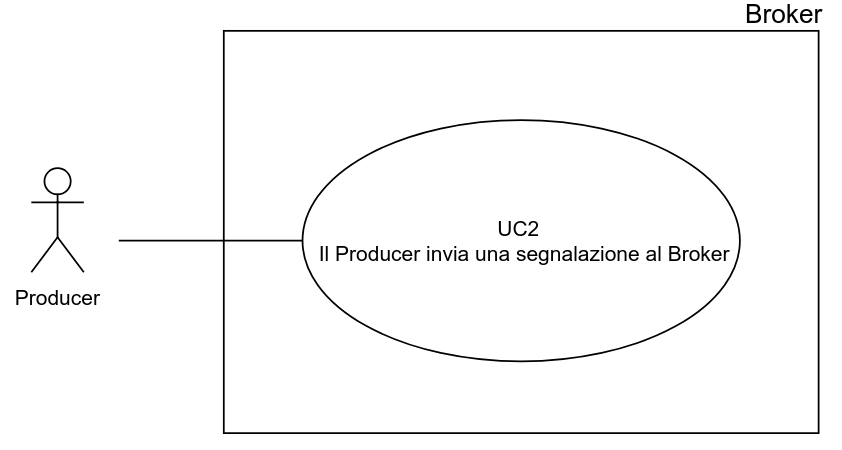
\includegraphics[width=0.7\textwidth]{img/UC2Producer.png}\\
		\caption{UC\theuccount - Il Producer invia una segnalazione al Broker}
	\end{figure}
	\begin{itemize}
		\item \textbf{Codice}: UC\theuccount.
		\item \textbf{Titolo}: il Producer invia una segnalazione al Broker.
		\item \textbf{Attori primari}: Producer.
		\item \textbf{Descrizione}: il Producer, dopo aver ricevuto una determinata segnalazione da Redmine/Gitlab, la inoltra al Broker in modo che possa istanziarne un Topic. Il sistema di riferimento qui è il Broker ed è interno al sistema Butterfly.
		\item \textbf{Precondizione}: il Producer ha ricevuto una segnalazione da inoltrare.
		\item \textbf{Postcondizione}: il Producer ha inviato al Broker la segnalazione.
		\item \textbf{Scenario principale}:
		\begin{enumerate}
			\item Il Producer procede all'invio della segnalazione
		\end{enumerate}
		 
	\end{itemize}

%Opzionale Sonarqube

\stepcounter{uccount}
\subsubsection{UC\theuccount\ - Il Consumer interroga il Broker}
	\begin{figure}[H]
		\centering
		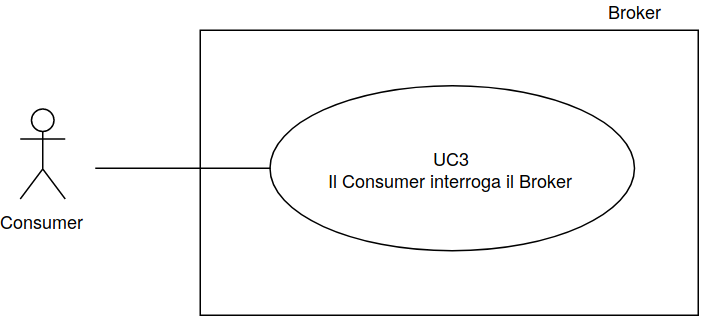
\includegraphics[width=\columnwidth]{img/UC3.png}\\
		\caption{UC\theuccount\ - Accesso}
	\end{figure}
	\begin{itemize}
		\item \textbf{Codice}: UC\theuccount.

		\item \textbf{Titolo}: il Consumer interroga il Broker.
		\item \textbf{Attori primari}: Consumer.
		\item \textbf{Descrizione}: il Consumer chiede al Broker di acquisire il messaggio da inoltrare verso il client della tecnologia specificata dall'utente finale. Il sistema di riferimento qui è Broker ed è interno al sistema Butterfly.
		\item \textbf{Precondizione}: il Broker ha un messaggio pronto ad essere inoltrato da un Consumer verso un client delle tecnologie con cui il sistema si interfaccia.
		\item \textbf{Postcondizione}: dopo aver recuperato il messaggio dal Broker il Consumer lo inoltra al client della tecnologia correlata in attesa con lo scopo l'utente finale lo legga.
		\item \textbf{Scenario principale}: 
			\begin{enumerate}
				\item Il Consumer richiede la segnalazione da inviare al client utilizzato dall'utente finale
			\end{enumerate}
	\end{itemize}

\stepcounter{uccount}
\subsubsection{UC\theuccount\ - Telegram/mail riceve un messaggio dal Consumer}
	\begin{figure}[H]
		\centering
			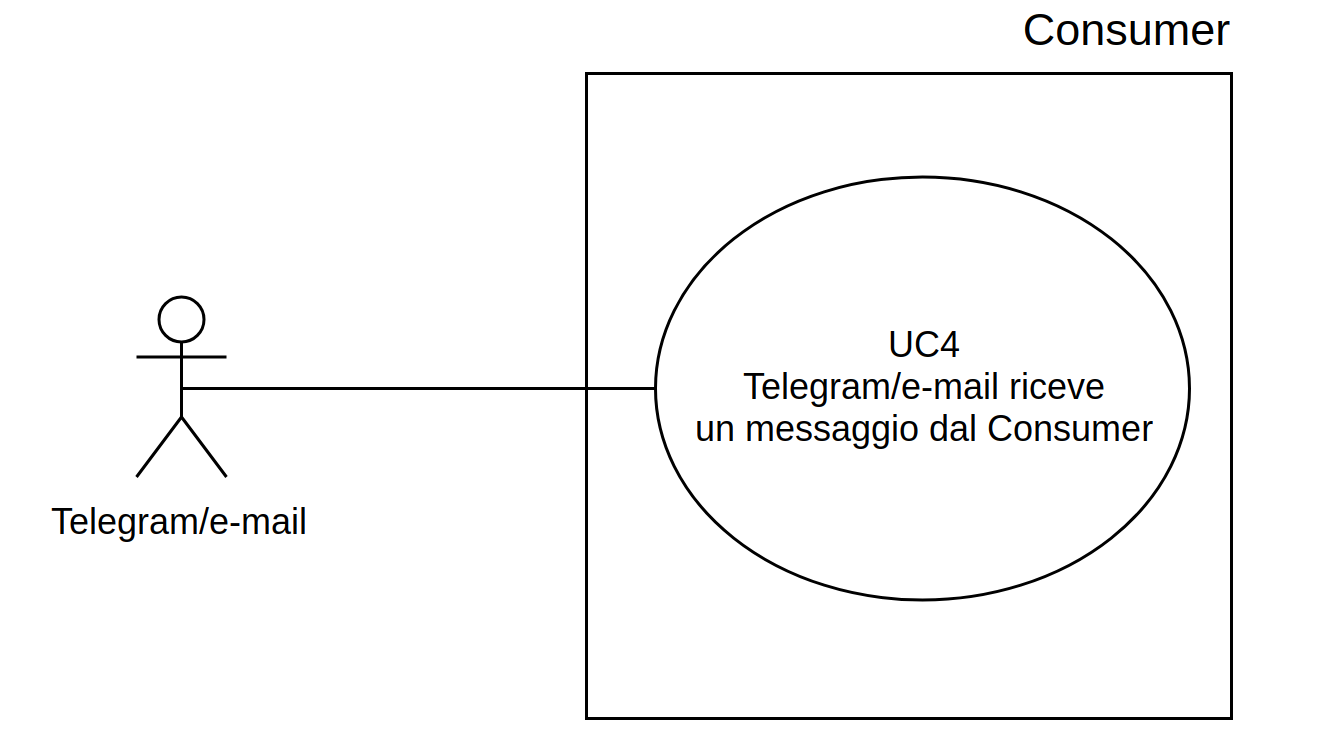
\includegraphics[width=\columnwidth]{img/UC4.png}\\
		\caption{UC\theuccount\ - Telegram/mail riceve un messaggio dal Consumer}
	\end{figure}
	\begin{itemize}
		\item \textbf{Codice}: UC\theuccount.
		\item \textbf{Titolo}: Telegram/mail riceve un messaggio dal Consumer.
		\item \textbf{Attori}: Telegram/server mail.
		\item \textbf{Descrizione}: il sistema di riferimento qui è il Consumer ed è interno al sistema Butterfly.
		Sebbene questo caso d'uso non sia del tutto corretto perchè l'attore Telegram/mail è un attore passivo, che riceve e non che agisce, è stato scelto di creare questo caso d'uso al fine di inserire la funzionalità "Il Consumer invia un messaggio a Telegram/mail". Ma scrivere un caso d'uso in tal modo sarebbe stato del tutto scorretto in quanto il sistema di riferimento in questo caso sarebbe stato Telegram/mail. Cosa non possibile dato che Telegram/mail è esterno a Butterfly e quindi non può essere considerato un suo sottosistema.
		\item \textbf{Precondizione}: il Consumer invia un messaggio a Telegram/server email in seguito a un'interrogazione del broker.
		\item \textbf{Postcondizione}: Telegram/server mail riceve il messaggio
		\item \textbf{Scenario principale}:
		\begin{enumerate}
			\item La ricezione del messaggio va a buon fine
		\end{enumerate} 
	\end{itemize}

% Opzionale Slack

\stepcounter{uccount}
\subsubsection{UC\theuccount\ - Accesso}
		\begin{figure}[H]
			\centering
				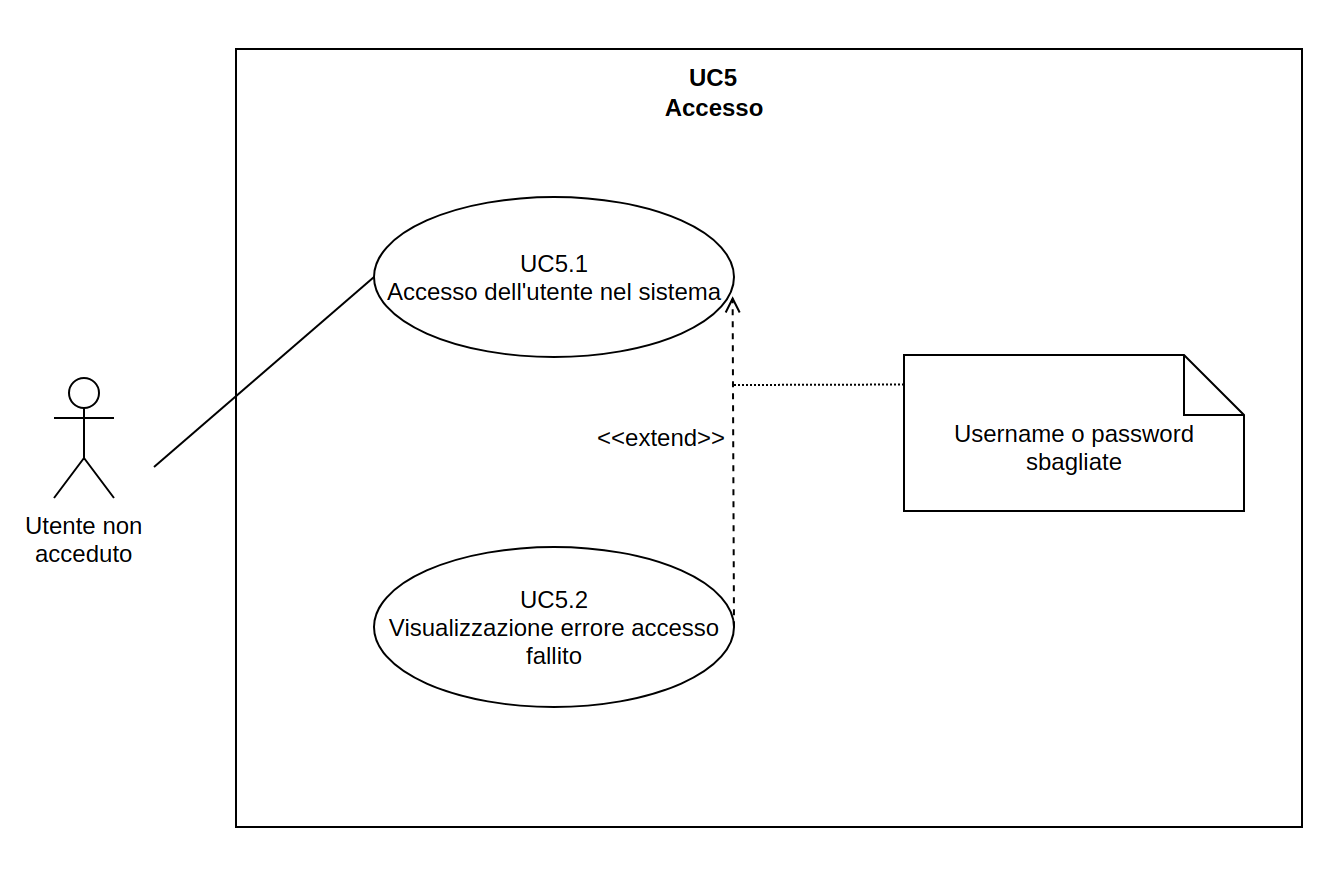
\includegraphics[width=\columnwidth]{img/UC5.png}\\
			\caption{UC\theuccount\ - Accesso}
		\end{figure}
	\begin{itemize}
		\item \textbf{Codice}: UC5
		\item \textbf{Titolo}: accesso
		\item \textbf{Attori primari}: utente non acceduto
		\item \textbf{Descrizione}: l'utente richiede di accedere al sistema attraverso un form dove inserisce username e password
		\item \textbf{Precondizione}: il sistema considera l’utilizzatore come un utente non acceduto
		\item \textbf{Postcondizione}: il sistema riconosce l'utilizzatore come utente acceduto
		\item \textbf{Scenario Principale}: l'utente non ancora riconosciuto dal sistema effettua l'accesso.
	\end{itemize}
	
	\paragraph{UC\theuccount.1 - Accesso dell'utente nel sistema}
		\begin{figure}[H]
			\centering
				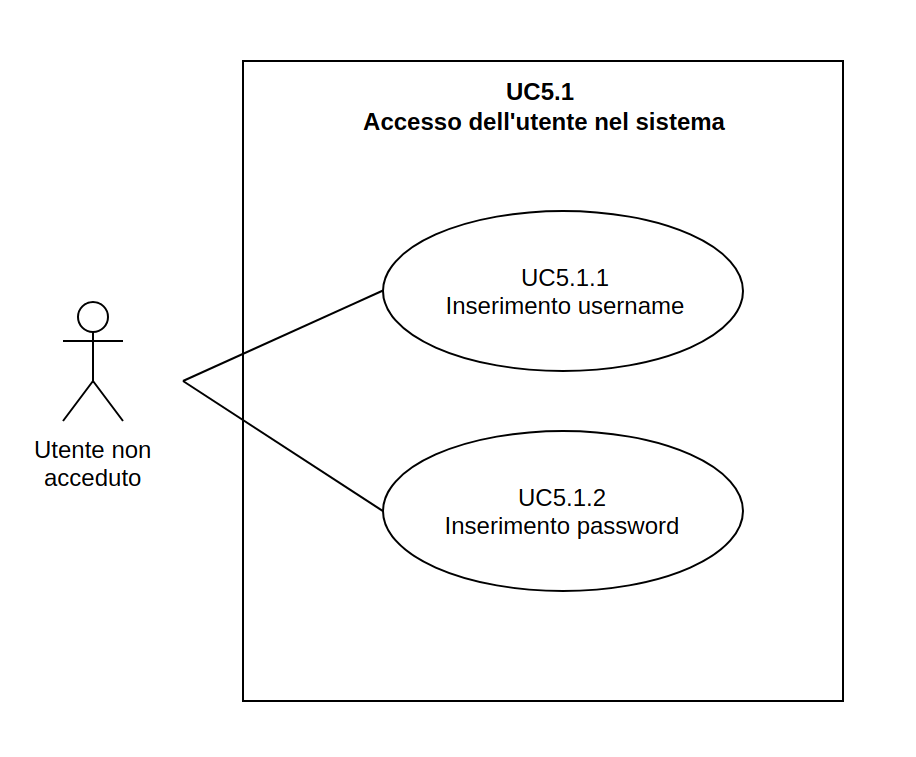
\includegraphics[width=\columnwidth]{img/UC5_1.png}\\
			\caption{UC\theuccount.1 - Accesso dell'utente nel sistema}
		\end{figure}
		\begin{itemize}
			\item \textbf{Codice}: UC\theuccount.1
			\item \textbf{Titolo}: accesso dell'utente nel sistema
			\item \textbf{Attori}: utente non acceduto
			\item \textbf{Descrizione}: l'utente attende l'autenticazione da parte del sistema
			\item \textbf{Precondizione}: il sistema riconosce l'utilizzatore come un utente non autenticato
			\item \textbf{Postcondizione}: il sistema riconosce l'utente autenticato con successo
			\item \textbf{Scenario Principale}: l’utente non ancora riconosciuto dal sistema richiede l'autenticazione
			\item \textbf{Estensioni}:
			\begin{enumerate}
				\item Nel caso in cui l'accesso non dovrebbe andare a buon fine viene visualizzato un errore avvisando l'utente [UC5.2].
			\end{enumerate}
	\end{itemize}

		\subparagraph{UC\theuccount.1.1 - Inserimento username}
			\begin{itemize}
				\item \textbf{Codice}: UC\theuccount.1.1
				\item \textbf{Titolo}: inserimento username
				\item \textbf{Attori}: utente non acceduto
				\item \textbf{Descrizione}: l'utente inserisce l'username
				\item \textbf{Precondizione}: il sistema offre l'interfaccia grafica adatta all'inserimento dell'username
				\item \textbf{Postcondizione}: l'utente ha inserito l'username desiderato
				\item \textbf{Scenario Principale}: l'utente inserisce l'username per autenticarsi.
			\end{itemize}
		
		\subparagraph{UC\theuccount.1.2 - Inserimento password}
			\begin{itemize}
				\item \textbf{Codice}: UC\theuccount.1.2	
				\item \textbf{Titolo}: inserimento password
				\item \textbf{Attori}: utente non acceduto
				\item \textbf{Descrizione}: l'utente inserisce la password
				\item \textbf{Precondizione}: il sistema offre l'interfaccia grafica adatta all'inserimento della password
				\item \textbf{Postcondizione}: l'utente ha inserito la password desiderata
				\item \textbf{Scenario Principale}: l'utente inserisce la password per autenticarsi.
			\end{itemize}
		
%Da aggiungere al limite più avanti
		
%		\subparagraph{UC5.1.2}
%			\begin{itemize}
%			\item \textbf{Codice}: UC6.1.2.
%			\item \textbf{Titolo}: inserimento password
%			\item \textbf{Attori}: utente non autenticato
%			\item \textbf{Descrizione}: l'utente inserisce la password
%			\item \textbf{Precondizione}: il sistema offre l'interfaccia grafica adatta all'inserimento della password
%			\item \textbf{Postcondizione}: l'utente ha inserito la password desiderata
%			\item \textbf{Scenario Principale}: l'utente inserisce la password per autenticarsi
%		\end{itemize}
	
	\paragraph{UC\theuccount.2 - Visualizzazione errore autenticazione fallita}
		\begin{itemize}
			\item \textbf{Titolo}: visualizzazione errore autenticazione fallita
			\item \textbf{Attori}: utente non autenticato
			\item \textbf{Descrizione}: l'utente viene avvisato che ha inserito username o password errate
			\item \textbf{Precondizione}: il sistema riceve una richiesta di accesso da parte di un utente che
			fornisce username o password sbagliate
			\item \textbf{Postcondizione}: il sistema comunica all'utilizzatore l'errore
			\item \textbf{Scenario Principale}: l'utente visualizza il messaggio d'errore.
		\end{itemize}


\stepcounter{uccount}
\subsubsection{UC\theuccount\ - Modifica delle preferenze}
	\begin{figure}[H]
		\centering
		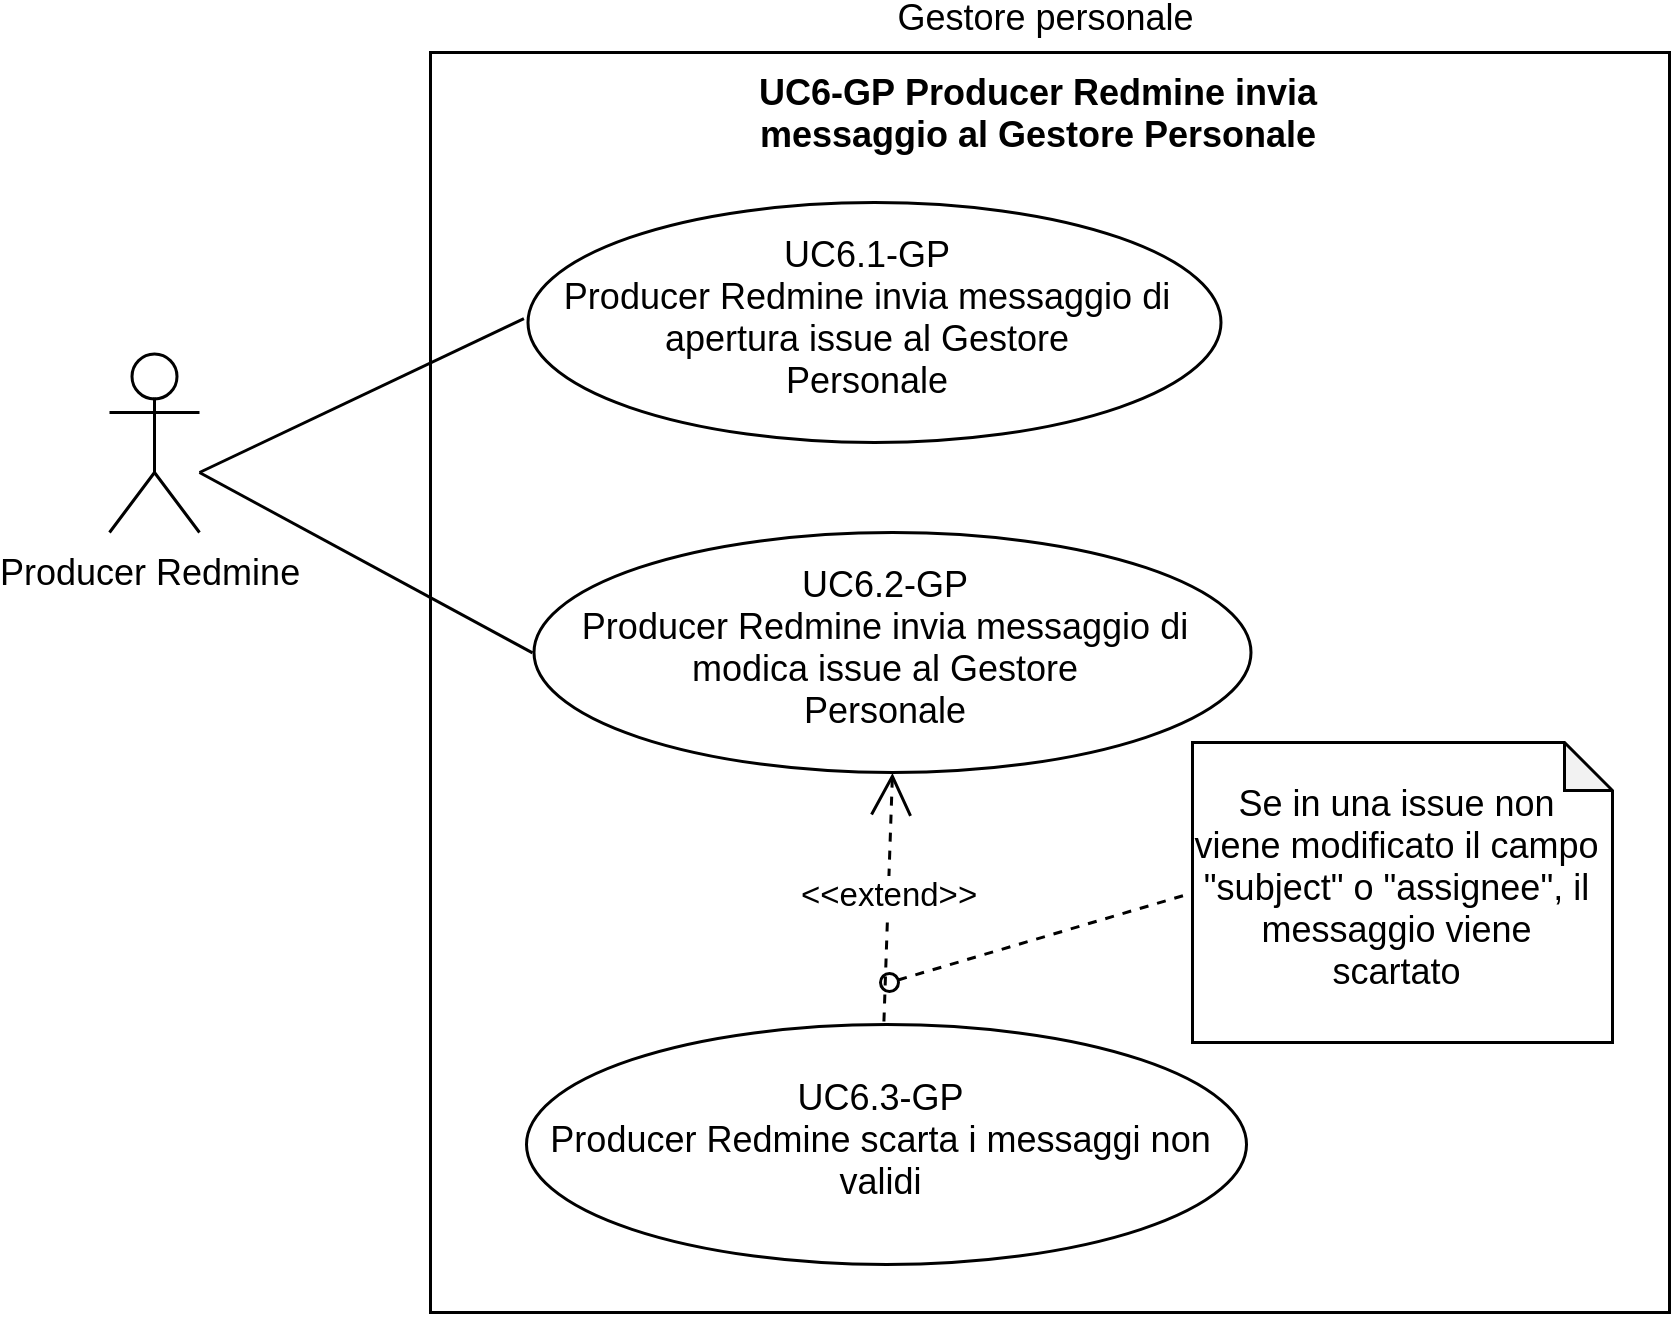
\includegraphics[width=\columnwidth]{img/UC6.png}\\
		\caption{UC\theuccount\ - Modifica delle preferenze}
	\end{figure}
	\begin{itemize}
		\item \textbf{Codice}: UC\theuccount.
		\item \textbf{Titolo}: modifica delle preferenze.
		\item \textbf{Attori}: Utente.
		\item \textbf{Descrizione}: attraverso un'interfaccia l'utente può modificare i vari parametri per configurare l'applicazione per le proprie esigenze. Il sistema di riferimento considerato è tutto \progetto.
		\item \textbf{Precondizione}: l'utente ha acceduto con le sue credenziali corrette nel sistema.
		\item \textbf{Postcondizione}: l'utente effettua zero o più modifiche nella configurazione personale dell'applicazione. 
		\item \textbf{Scenario Principale}: L'utente ha la possibilità di portare delle modifiche alle sue preferenze all'interno dell'applicazione \progetto.
	\end{itemize}



	\paragraph{UC\theuccount.1 - Aggiunta preferenze}
		\begin{figure}[H]
			\centering
			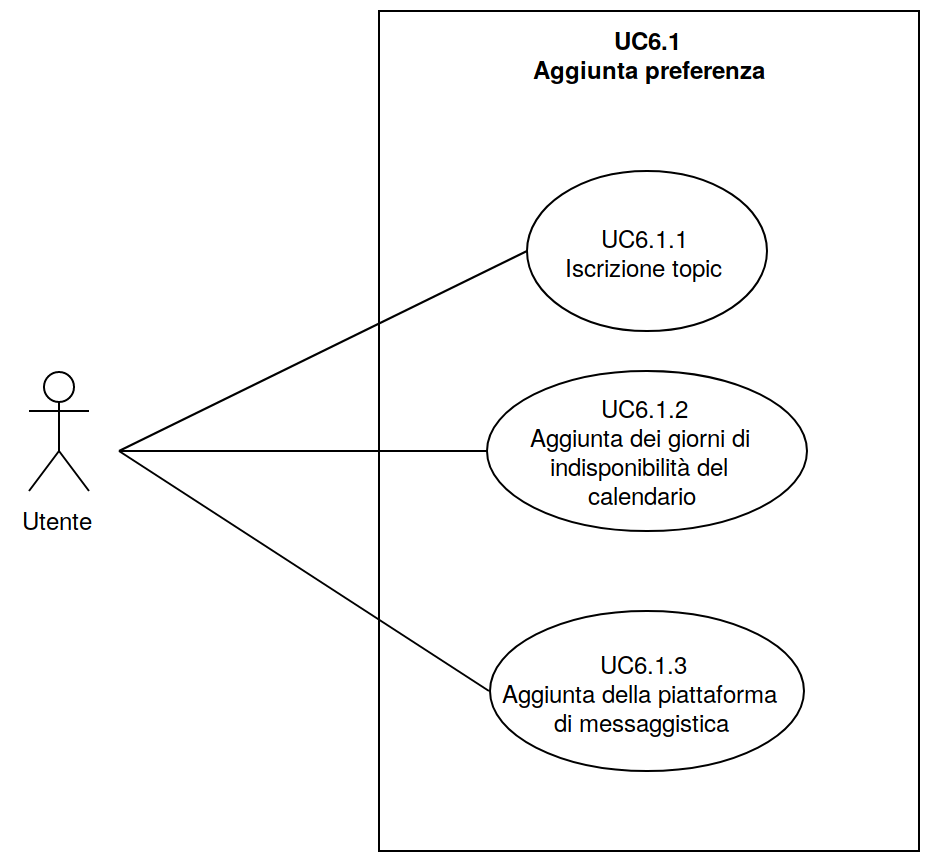
\includegraphics[width=\columnwidth]{img/UC6_1.png}\\
			\caption{UC\theuccount.1 - Aggiunta preferenze}
		\end{figure}
	\begin{itemize}
		\item \textbf{Codice}: UC\theuccount.1.
		\item \textbf{Titolo}: aggiunta preferenze.
		\item \textbf{Descrizione}: l'utente, date le varie opzioni per configurare \progetto, aggiunge una preferenza tra topic, giorni di calendario e piattaforme di messaggistica.
		\item \textbf{Precondizione}: l'utente ha acceduto con le sue credenziali corrette nel sistema e non ha selezionato tutte le preferenze possibili proposte da \progetto.
		\item \textbf{Postcondizione}: lo nuova configurazione contiene una o più preferenza in aggiunta rispetto alla quella precedente.
		\item \textbf{Scenario principale}: l'utente può scegliere, tra le varie opzioni disponibili disponi, quale aggiungere alla sua configurazione personale.
	\end{itemize}
	
	\subparagraph{UC\theuccount.1.1 - Iscrizione topic}
	\begin{itemize}
		\item \textbf{Codice}: UC\theuccount.1.1.
		\item \textbf{Titolo}: iscrizione topic.
		\item \textbf{Descrizione}: data la lista di topic presenti già inserita precedentemente, l'utente seleziona quelli a cui è interessato volendone ricevere una notifica. I topic sono divisi per categoria comprendendo etichette o parole chiave stabilite in precedenza.
		\item \textbf{Precondizione}: l'utente ha acceduto con le sue credenziali corrette nel sistema e non ha selezionato tutte le preferenze possibili proposte da \progetto.
		\item \textbf{Postcondizione}: il numero di topic a cui è interessato l'utente è aumentato.
		\item \textbf{Scenario principale}: l'utente aggiunge un topic dalla lista proposta dall'applicazione \progetto.
	\end{itemize}
		
			
	\subparagraph{UC\theuccount.1.2 - Aggiunta giorno irreperibilità nel calendario} 
	\begin{itemize}
		\item \textbf{Codice}: UC\theuccount.1.2.
		\item \textbf{Titolo}: aggiunta dei giorni di indisponibilità nel calendario.
		\item \textbf{Descrizione}: dato il calendario lavorativo, l'utente aggiunge i giorni in cui è reperibile e non vuole ricevere notifiche.
		\item \textbf{Precondizione}: l'utente ha acceduto con le sue credenziali corrette nel sistema e non ha selezionato tutte le preferenze possibili proposte da \progetto.
		\item \textbf{Postcondizione}: il numero di giorni in cui l'utente non si rende disponibile.
		\item \textbf{Scenario principale}: l'utente aggiunge le date di calendario in cui non è reperibile.
	\end{itemize}
			
	\subparagraph{UC\theuccount.1.3 - Aggiunta della piattaforma di messaggistica}
	\begin{itemize}
		\item \textbf{Codice}: UC\theuccount.1.3.
		\item \textbf{Titolo}:aggiunta della piattaforma di messaggistica.
		\item \textbf{Descrizione}: dalla lista delle piattaforme di messaggistica l'utente aggiunge quelle da cui vuole ricevere le notifiche.
		\item \textbf{Precondizione}: l'utente ha acceduto con le sue credenziali corrette nel sistema e non ha selezionato tutte le preferenze possibili proposte da \progetto.
		\item \textbf{Postcondizione}: il numero di piattaforme di messaggistica selezionate dall'utente è aumentato.
		\item \textbf{Scenario principale}: l'utente aggiunge le piattaforme di messaggistica da un elenco già fornito. 
		%telegram: nickname e mail sono già salvati nel DB
	\end{itemize}
			



	\paragraph{UC\theuccount.2 - Rimozione preferenza}
		\begin{figure}[H]
			\centering
			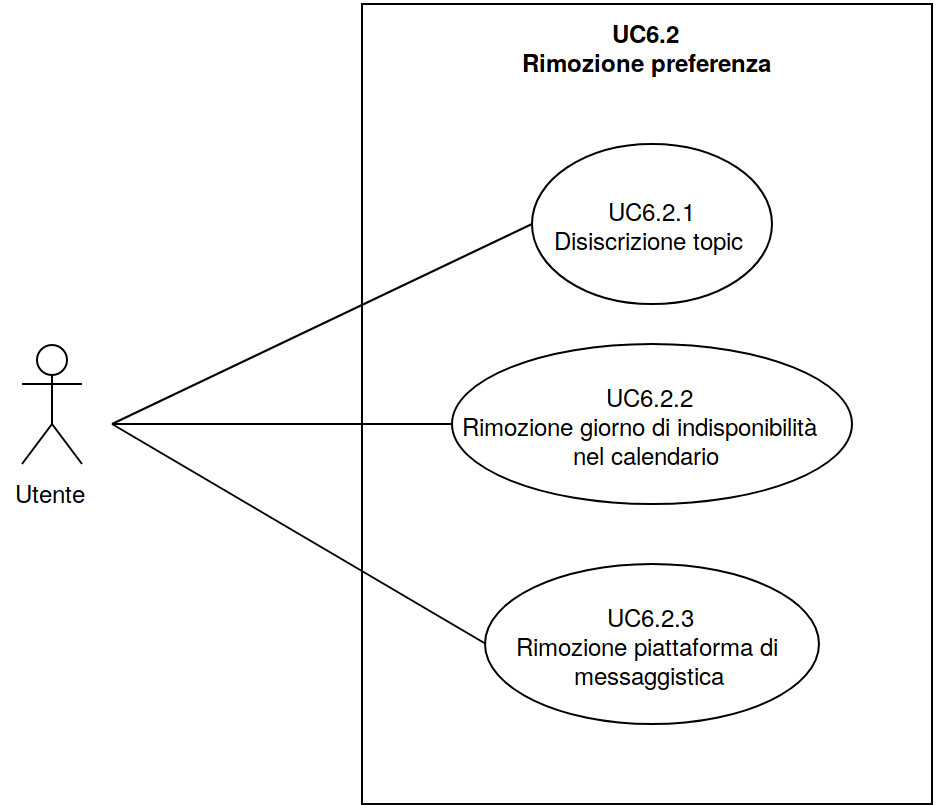
\includegraphics[width=\columnwidth]{img/UC6_2.png}\\
			\caption{UC\theuccount.2 - Rimozione preferenza}
		\end{figure}
	\begin{itemize}
		\item \textbf{Codice}: UC\theuccount.2.
		\item \textbf{Titolo}: rimozione preferenza.
		\item \textbf{Descrizione}: l'utente, dopo aver selezionato delle preferenze dalle opzioni di configurazione, ne rimuove una o di più. Le preferenze consistono in topic, date di calendario e piattaforme di messaggistica.
		\item \textbf{Precondizione}: l'utente ha acceduto con le credenziali nel sistema ed è presente almeno una preferenza selezionata tra quelle proposte da \progetto.
		\item \textbf{Postcondizione}: la nuova configurazione contiene una o più configurazioni in meno rispetto a quella precedente.
		\item \textbf{Scenario principale}: l'utente selezione tra le preferenze già scelte precedentemente quale rimuovere.
	\end{itemize}
	
	
	\subparagraph{UC\theuccount.2.1 - Disiscrizione topic}
	\begin{itemize}
		\item \textbf{Codice}: UC\theuccount.2.1.
		\item \textbf{Titolo}: disiscrizione topic.
		\item \textbf{Descrizione}: l'utente di disiscrive da un topic da uno o o più topic dai quali prima riceveva delle notifiche.
		\item \textbf{Precondizione}: l'utente ha acceduto con le credenziali nel sistema ed è presente almeno una preferenza selezionata tra quelle proposte da \progetto.
		\item \textbf{Postcondizione}: il numero di topic a cui è iscritto un utente è diminuito.
		\item \textbf{Scenario principale}: l'utente seleziona i topic a cui si era iscritto precedentemente per disicriversi.
	\end{itemize}
	
			
	\subparagraph{UC\theuccount.2.2 - Rimozione giorno irreperibilità nel calendario}
	\begin{itemize}
		\item \textbf{Codice}: UC\theuccount.2.2.
		\item \textbf{Titolo}: rimozione giorno irreperibilità nel calendario.
		\item \textbf{Descrizione}: l'utente rimuove i giorni di calendario in cui precedentemente non era reperibile.
		\item \textbf{Precondizione}: l'utente ha acceduto con le credenziali nel sistema ed è presente almeno una preferenza selezionata tra quelle proposte da \progetto.
		\item \textbf{Postcondizione}: il numero di giorni di calendario in cui l'utente non è reperibile è diminuito.
		\item \textbf{Scenario principale}: l'utente, dopo aver visto i giorni in cui si era segnato non reperibile, ne rimuove alcuni rendendosi disponibile in quelle date.
	\end{itemize}
			
			
	\subparagraph{UC\theuccount.2.3 - Rimozione piattaforma di messaggistica}
	\begin{itemize}
		\item \textbf{Codice}: UC\theuccount.2.3.
		\item \textbf{Titolo}: rimozione piattaforma di messaggistica.
		\item \textbf{Descrizione}: l'utente rimuove le piattaforme di messaggistica dalle quali non vuole più ricevere notifiche tramite \progetto.
		\item \textbf{Precondizione}: l'utente ha acceduto con le credenziali nel sistema ed è presente almeno una preferenza selezionata tra quelle proposte da \progetto.
		\item \textbf{Postcondizione}: il numero di piattaforme di messaggistica da cui l'utente vuole ricevere notifiche è diminuito.
		\item \textbf{Scenario principale}: l'utente seleziona da un elenco già presente le piattaforme di messaggistica che aveva precedentemente selezionato da cui non vuole più ricevere notifiche tramite \progetto.
	\end{itemize}

%Da tenere in considerazione per la pagina da creare più avanti	
%	\paragraph{UC7.4}
%	Annullo le modifiche fatte

		
